\documentclass{../../PublicResources/DocClass}

    \DocumentTitle{「研究生入学考试」学习笔记}
    \DocumentCreatedDate{2020/12/19}

    \LinkBlogPost{}
    \LinkPDFSource{}
    \LinkVideo{}

    \AuthorName{Mr. Kin}
    \AuthorEmail{im.misterkin@gmail.com}
    \AuthorBlog{https://mister-kin.github.io/}

\begin{document}
    \pagenumbering{Roman} % 大写罗马字母样式页码。
    \maketitle
    \addcontentsline{toc}{chapter}{封面}
    \frontmatter
    \phantomsection
\begin{center}
    {\bfseries\sffamily\Large 关于作者}
\end{center}
\addcontentsline{toc}{chapter}{关于作者}

\subsection*{\bfseries \sffamily 关于我}
\begin{wrapfigure}[3]{L}{60pt}
    \vspace*{-20pt}
    \centering
    
\includegraphics{kin-logo}
\end{wrapfigure}
\textbf{Mr. Kin},广东客家仁,程序猿,CG和游戏爱好者,一枚极客。翻译UP主,个人UP主。不定时在B站直播日常:码代码,码博客,翻译,做视频,做教程。 ($\vartheta$$\bullet$\_$\bullet$)$\vartheta$ \hyperlink{follow}{\emph{(点击关注我!)}}

\subsection*{\bfseries \sffamily 开源建设}

\noindent {\bfseries \sffamily 开源软件的中文化翻译}

\begin{itemize}
    \item \href{https://docs.krita.org/zh_CN/}{Krita手册}:2018.8.5 - \href{https://crowdin.com/profile}{2019.4.23}
    \item \href{https://docs.blender.org/manual/zh-hans/latest/}{Blender手册}:2019.7.20 - \href{https://www.blendercn.org/5812.html?tdsourcetag=s_pctim_aiomsg}{2019.9.4} - 至今(\href{https://developer.blender.org/p/Mr_Kin/}{翻译维护})
\end{itemize}

\subsection*{\bfseries \sffamily \hypertarget{contact}{联系方式}}
\vspace*{-1ex}
\noindent {\footnotesize \color{red} \em 注:联系时请注明身份,谢谢!}

\begin{itemize}
    \item QQ:\href{tencent://AddContact/?fromId=45&fromSubId=1&subcmd=all&uin=2312463626&website=www.oicqzone.com}{2312463626}\emph{\color{red}(点击号码加好友)}
    \item 邮箱:2312463626@qq.com ; im.misterkin@gmail.com
\end{itemize}

\subsection*{\bfseries \sffamily \hypertarget{follow}{关注渠道}}
\vspace*{-1ex}
\noindent {\footnotesize \color{red} \em 注:点击文字即可跳转关注!}
\vspace*{-2ex}

\begin{figure}[htbp]
    \centering
    
\includegraphics[scale=0.2]{WechatOfficialAccounts.png}
\end{figure}
\vspace*{-4ex}

\begin{figure}[htbp]
    \centering
    \begin{minipage}[t]{0.2\textwidth}
        \centering
        \caption*{\href{https://mister-kin.github.io}{博客 - Blog}}
        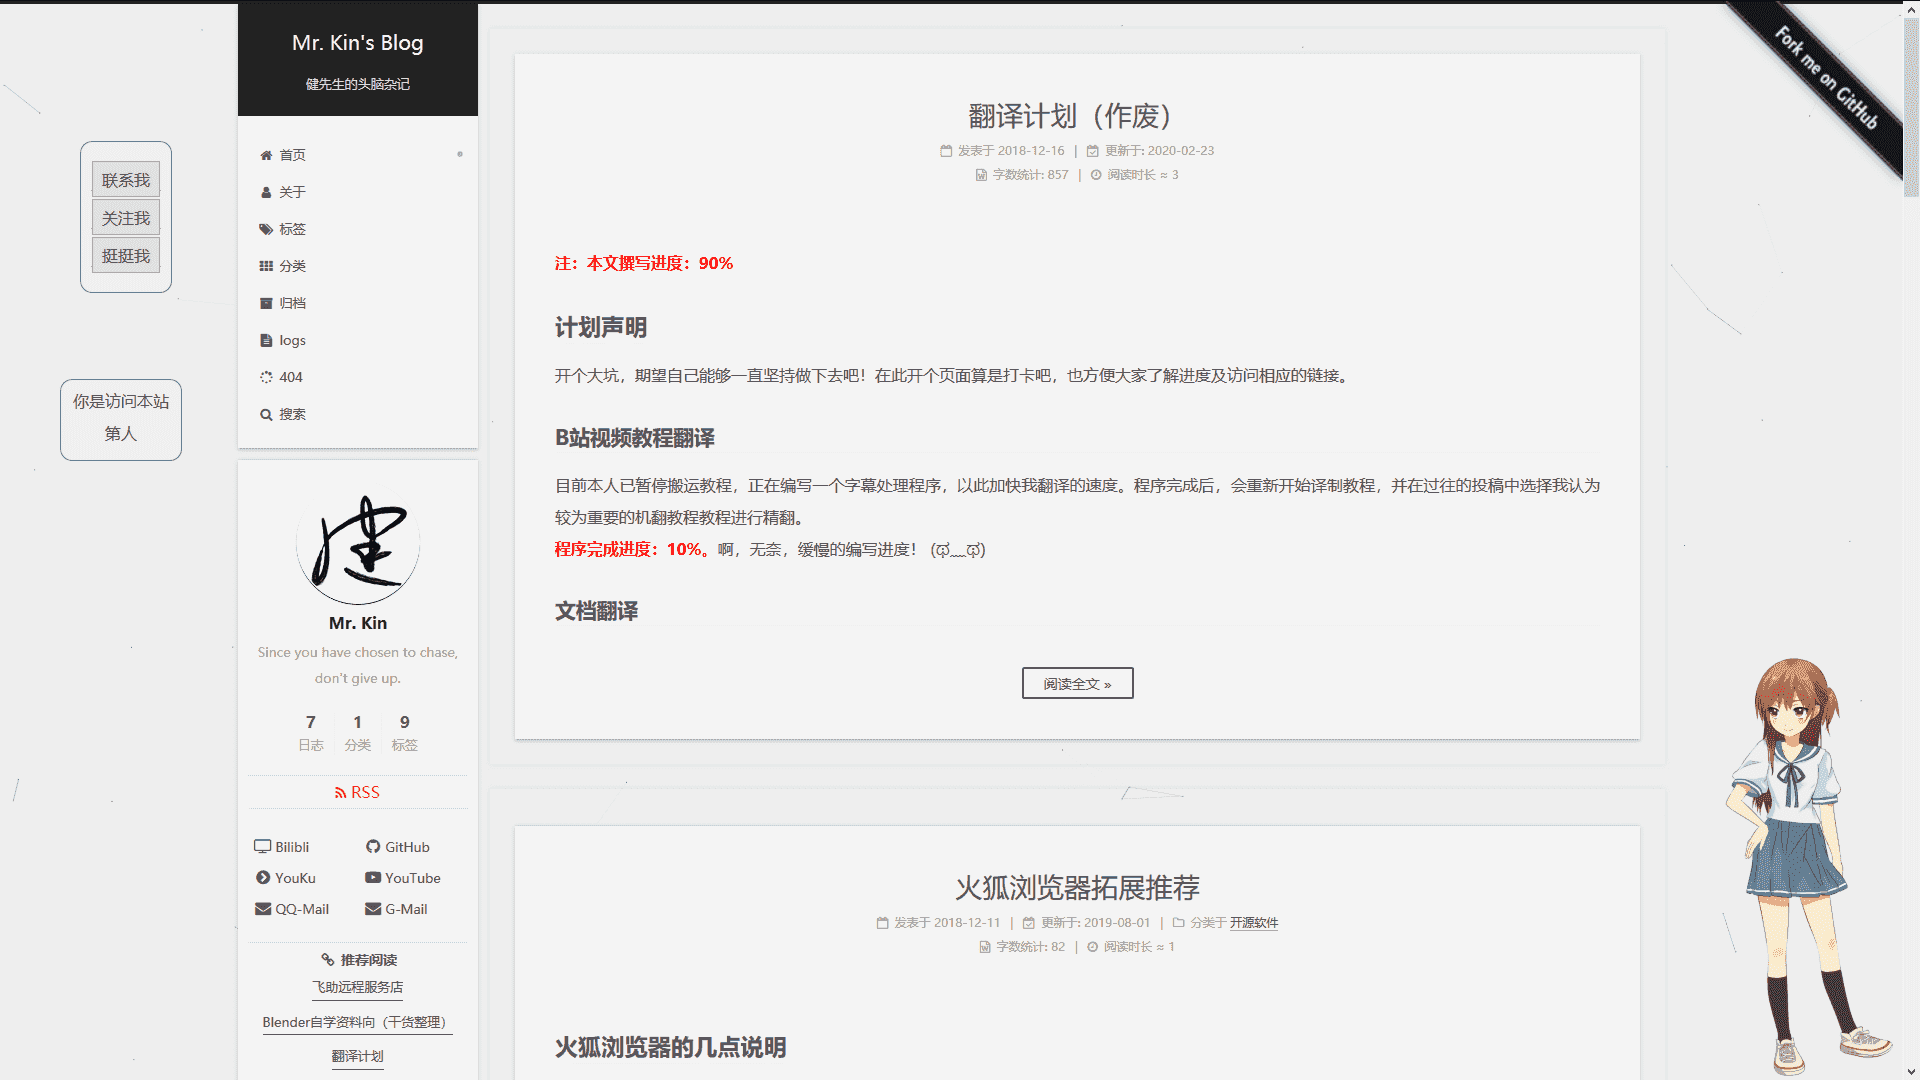
\includegraphics[scale=0.055]{Blog}
    \end{minipage}
    \qquad
    \begin{minipage}[t]{0.2\textwidth}
        \centering
        \caption*{\href{https://github.com/mister-kin}{Github}}
        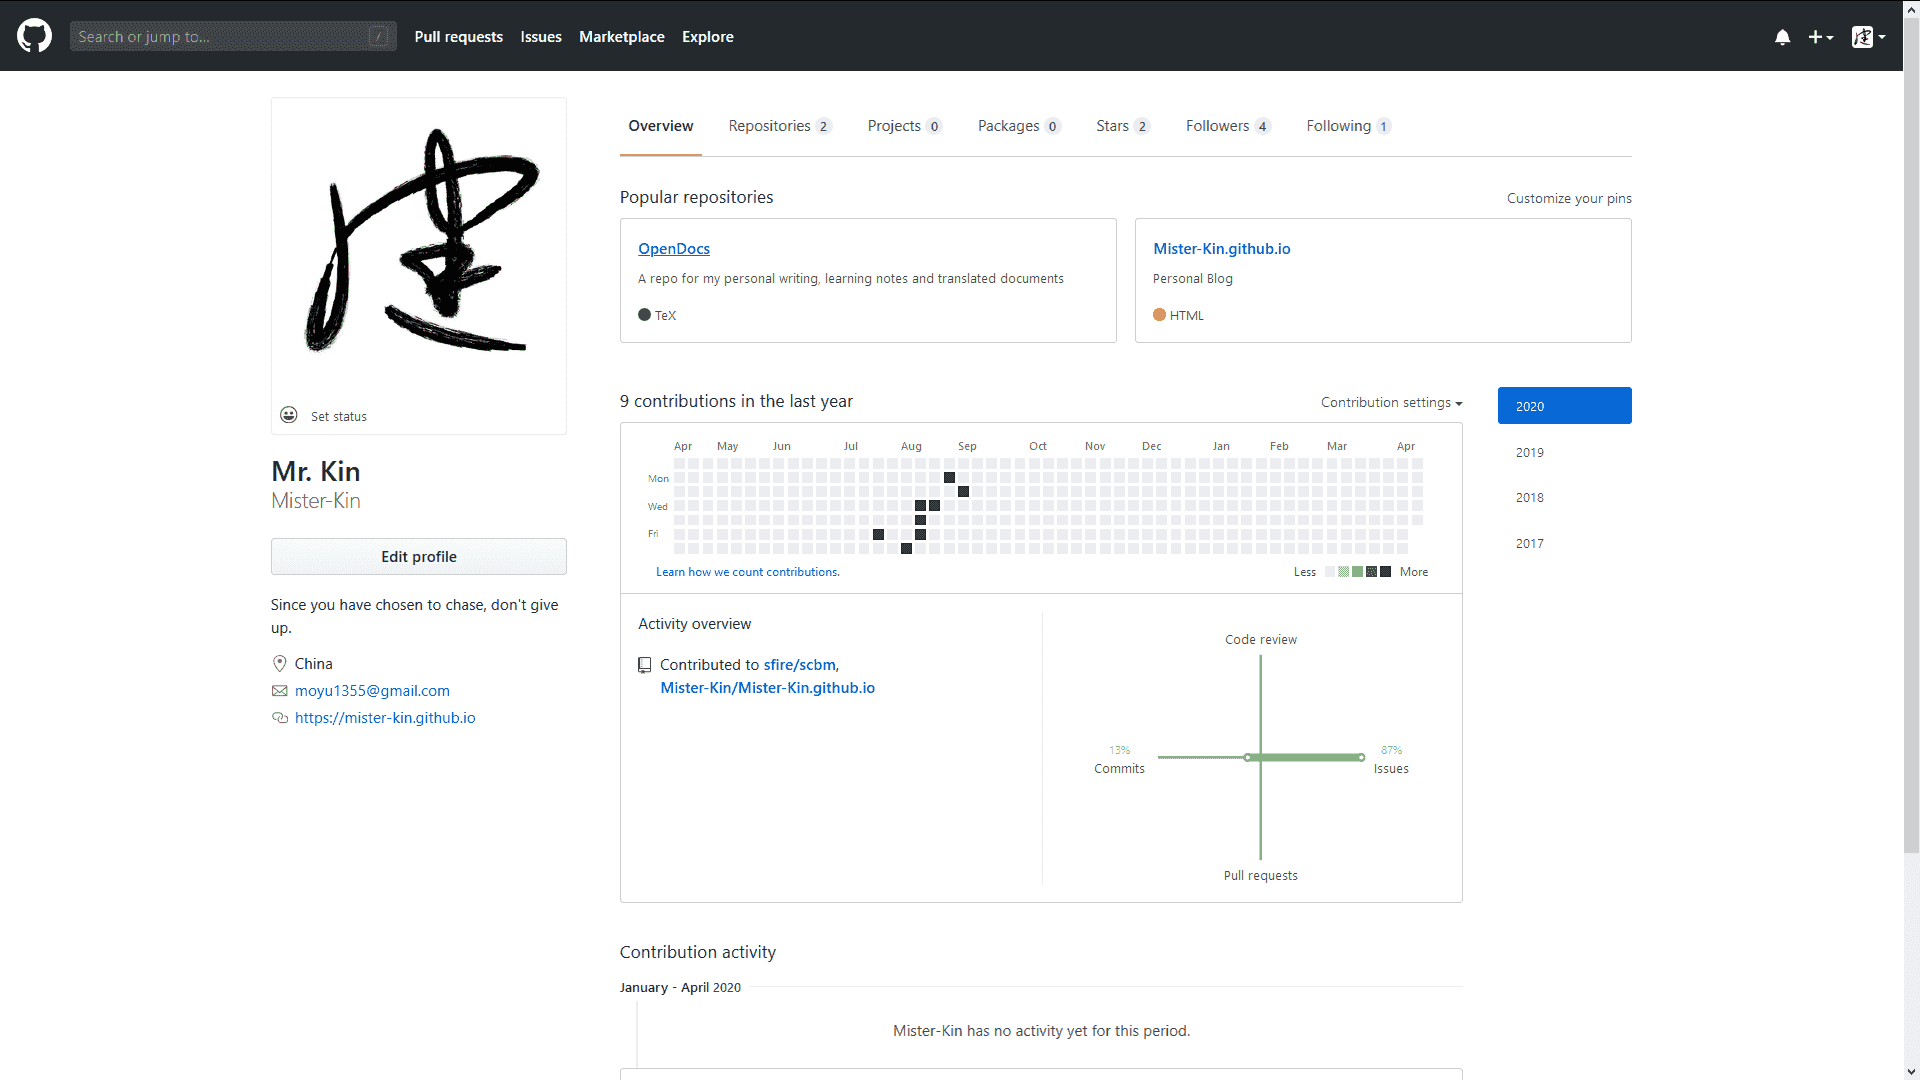
\includegraphics[scale=0.055]{Github}
    \end{minipage}
    \qquad
    \begin{minipage}[t]{0.2\textwidth}
        \centering
        \caption*{\href{https://weibo.com/6270111192/profile?topnav=1&wvr=6&is_all=1}{微博 - Weibo}}
        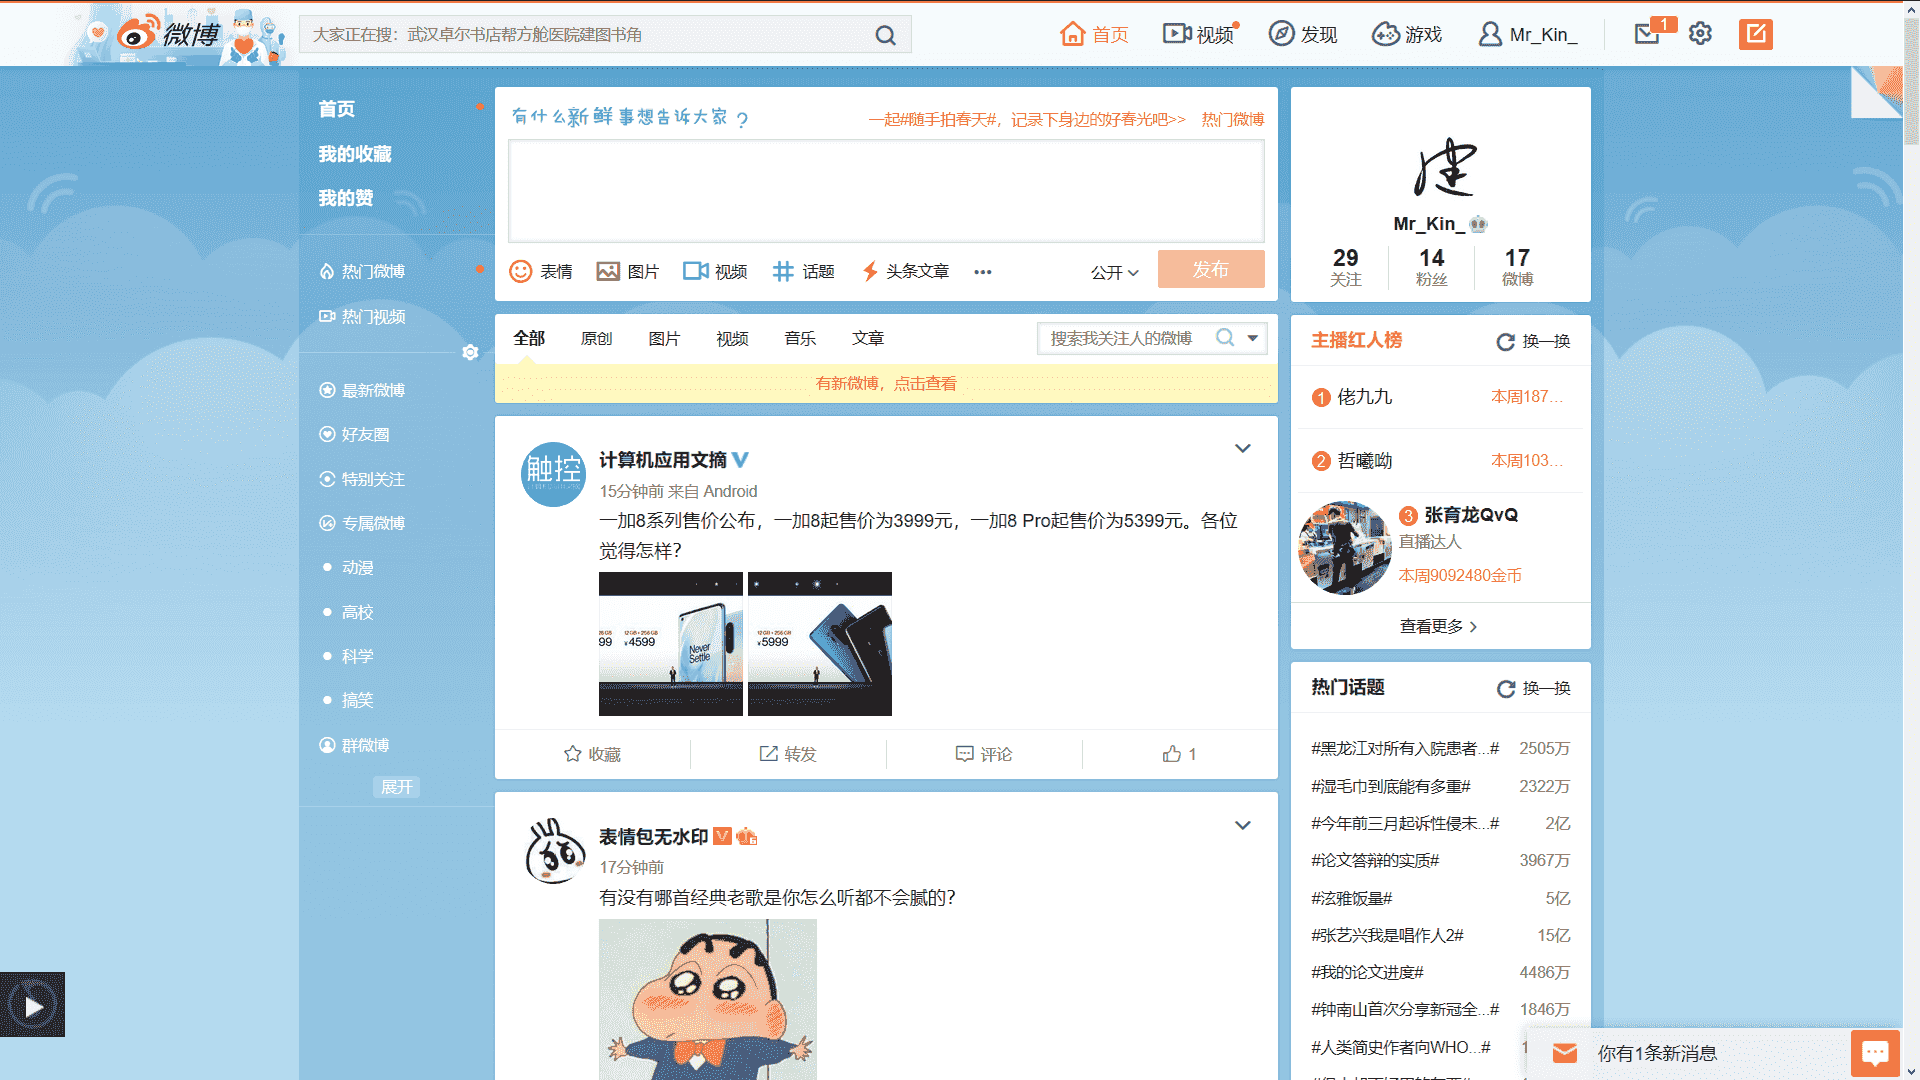
\includegraphics[scale=0.055]{Weibo}
    \end{minipage}
    \qquad
    \begin{minipage}[t]{0.2\textwidth}
        \centering
        \caption*{\href{https://www.zhihu.com/people/drwu-94}{知乎 - Zhihu}}
        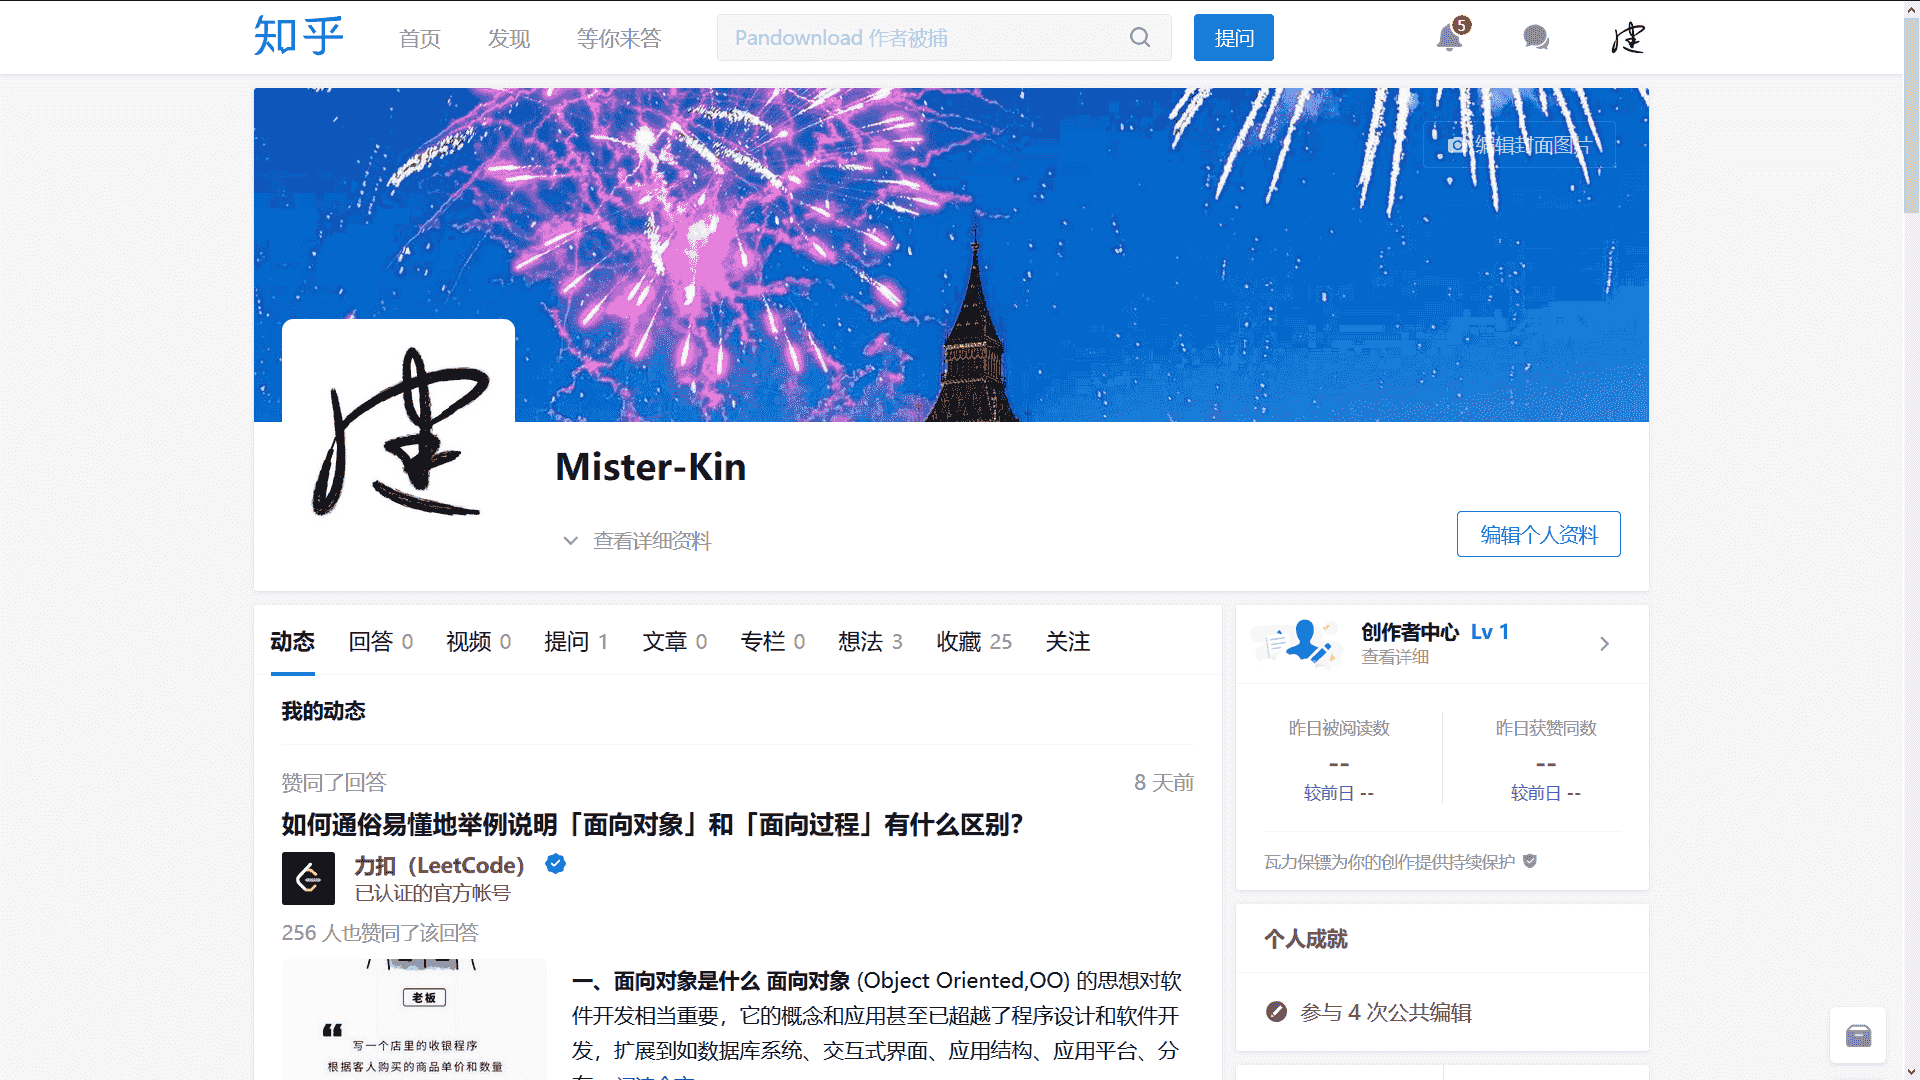
\includegraphics[scale=0.055]{Zhihu}
    \end{minipage}

    \vspace*{3ex}

    \begin{minipage}[t]{0.2\textwidth}
        \centering
        \caption*{\href{http://space.bilibili.com/17025250?}{B站 - Bilibili}}
        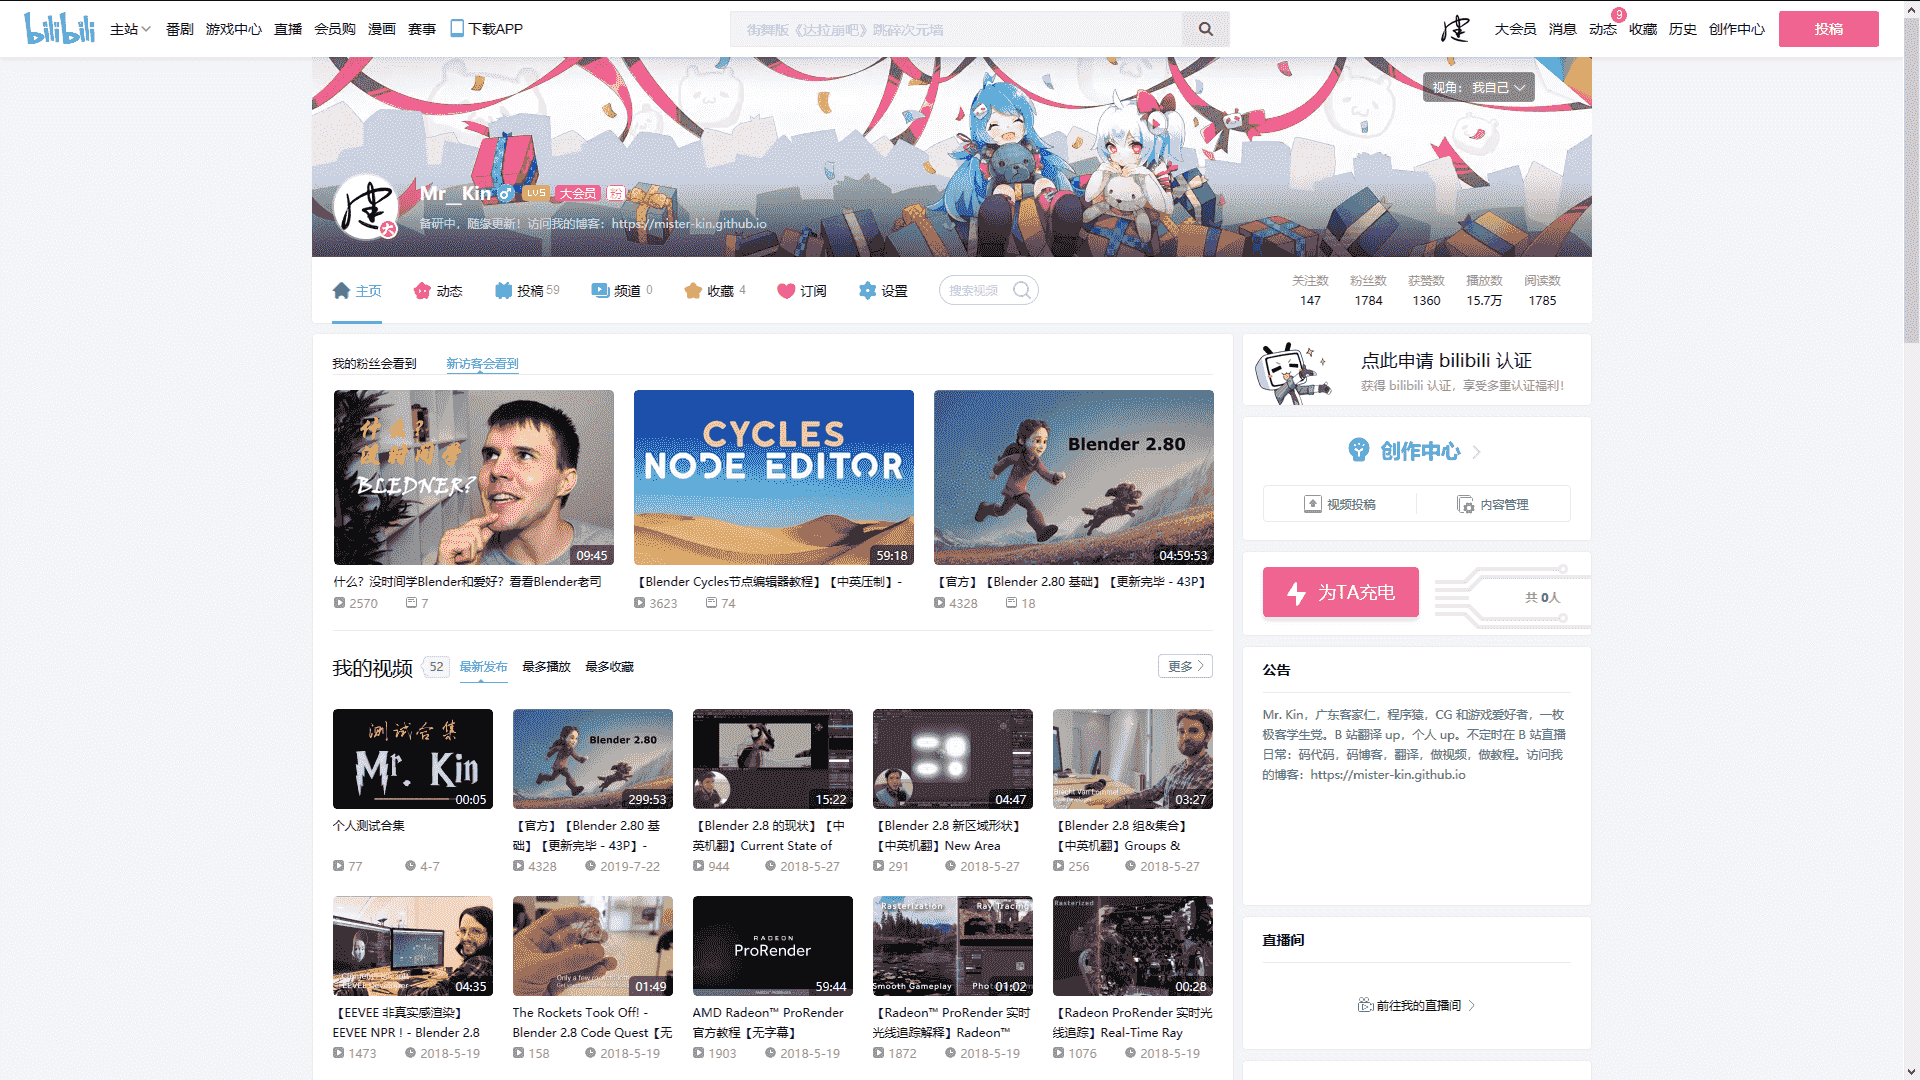
\includegraphics[scale=0.055]{Bilibili}
    \end{minipage}
    \qquad
    \begin{minipage}[t]{0.2\textwidth}
        \centering
        \caption*{\href{http://i.youku.com/i/UNjA3MTk5Mjgw?spm=a2hzp.8253869.0.0}{优酷 - Youku}}
        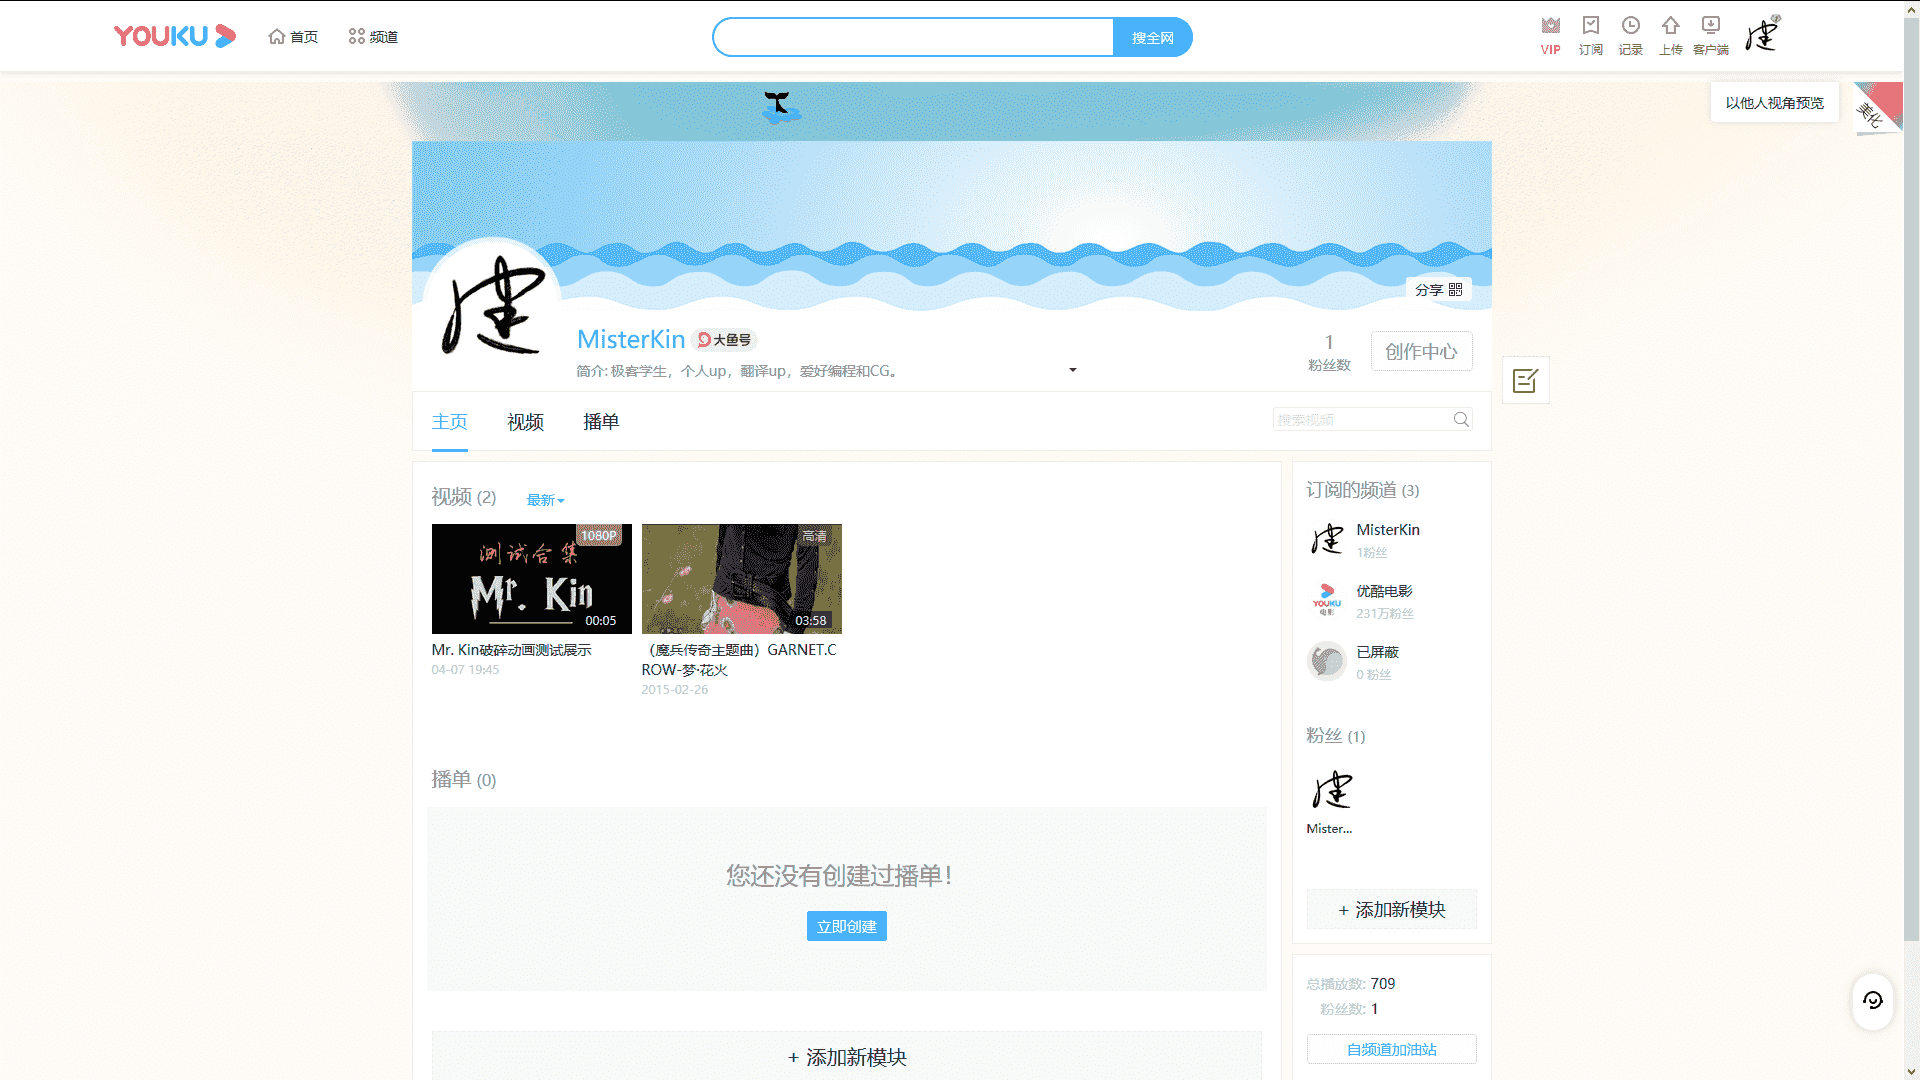
\includegraphics[scale=0.055]{Youku}
    \end{minipage}
    \qquad
    \begin{minipage}[t]{0.2\textwidth}
        \centering
        \caption*{\href{https://www.toutiao.com/c/user/835254071079053/\#mid=1663279303982091}{头条 - Headline}}
        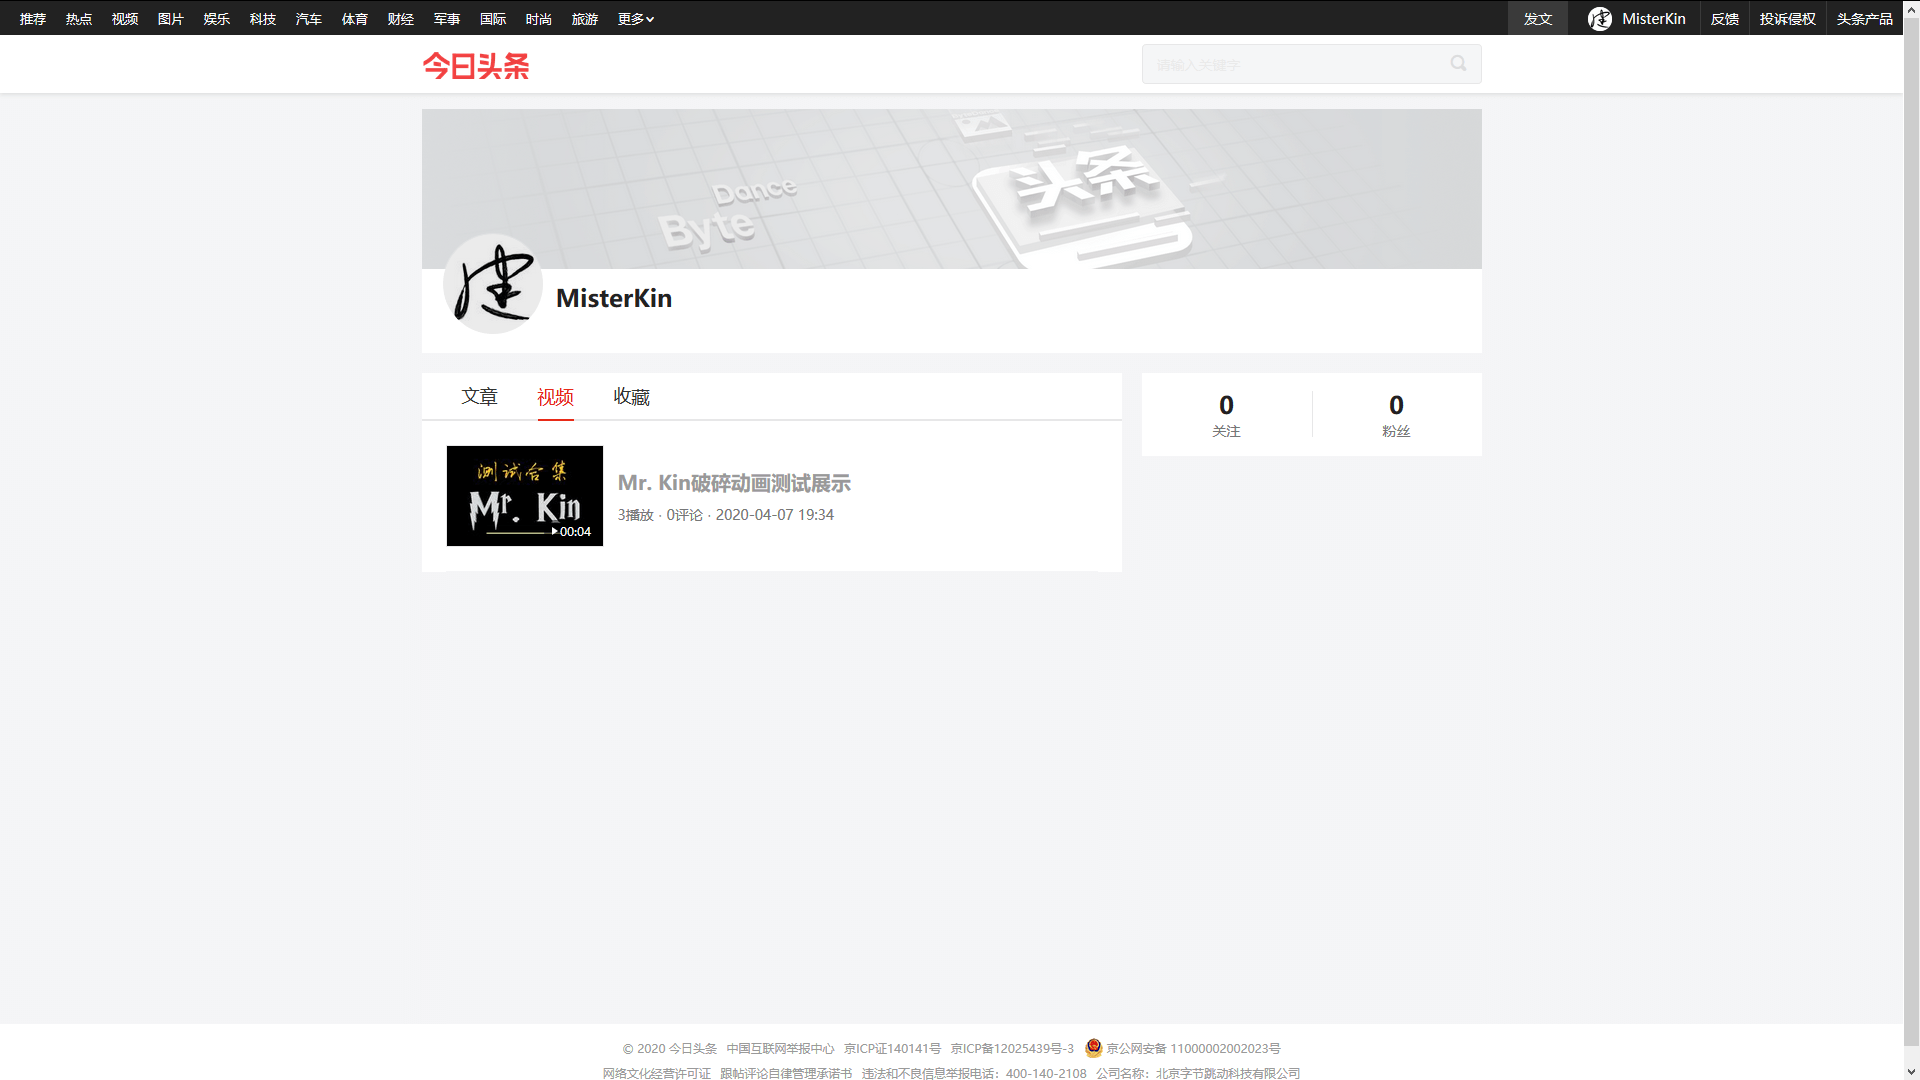
\includegraphics[scale=0.055]{Headline}
    \end{minipage}
    \qquad
    \begin{minipage}[t]{0.2\textwidth}
        \centering
        \caption*{\href{https://www.youtube.com/channel/UCXqjfWLzMlRKxGC8syWj17Q?view_as=public}{油管 - Youtube}}
        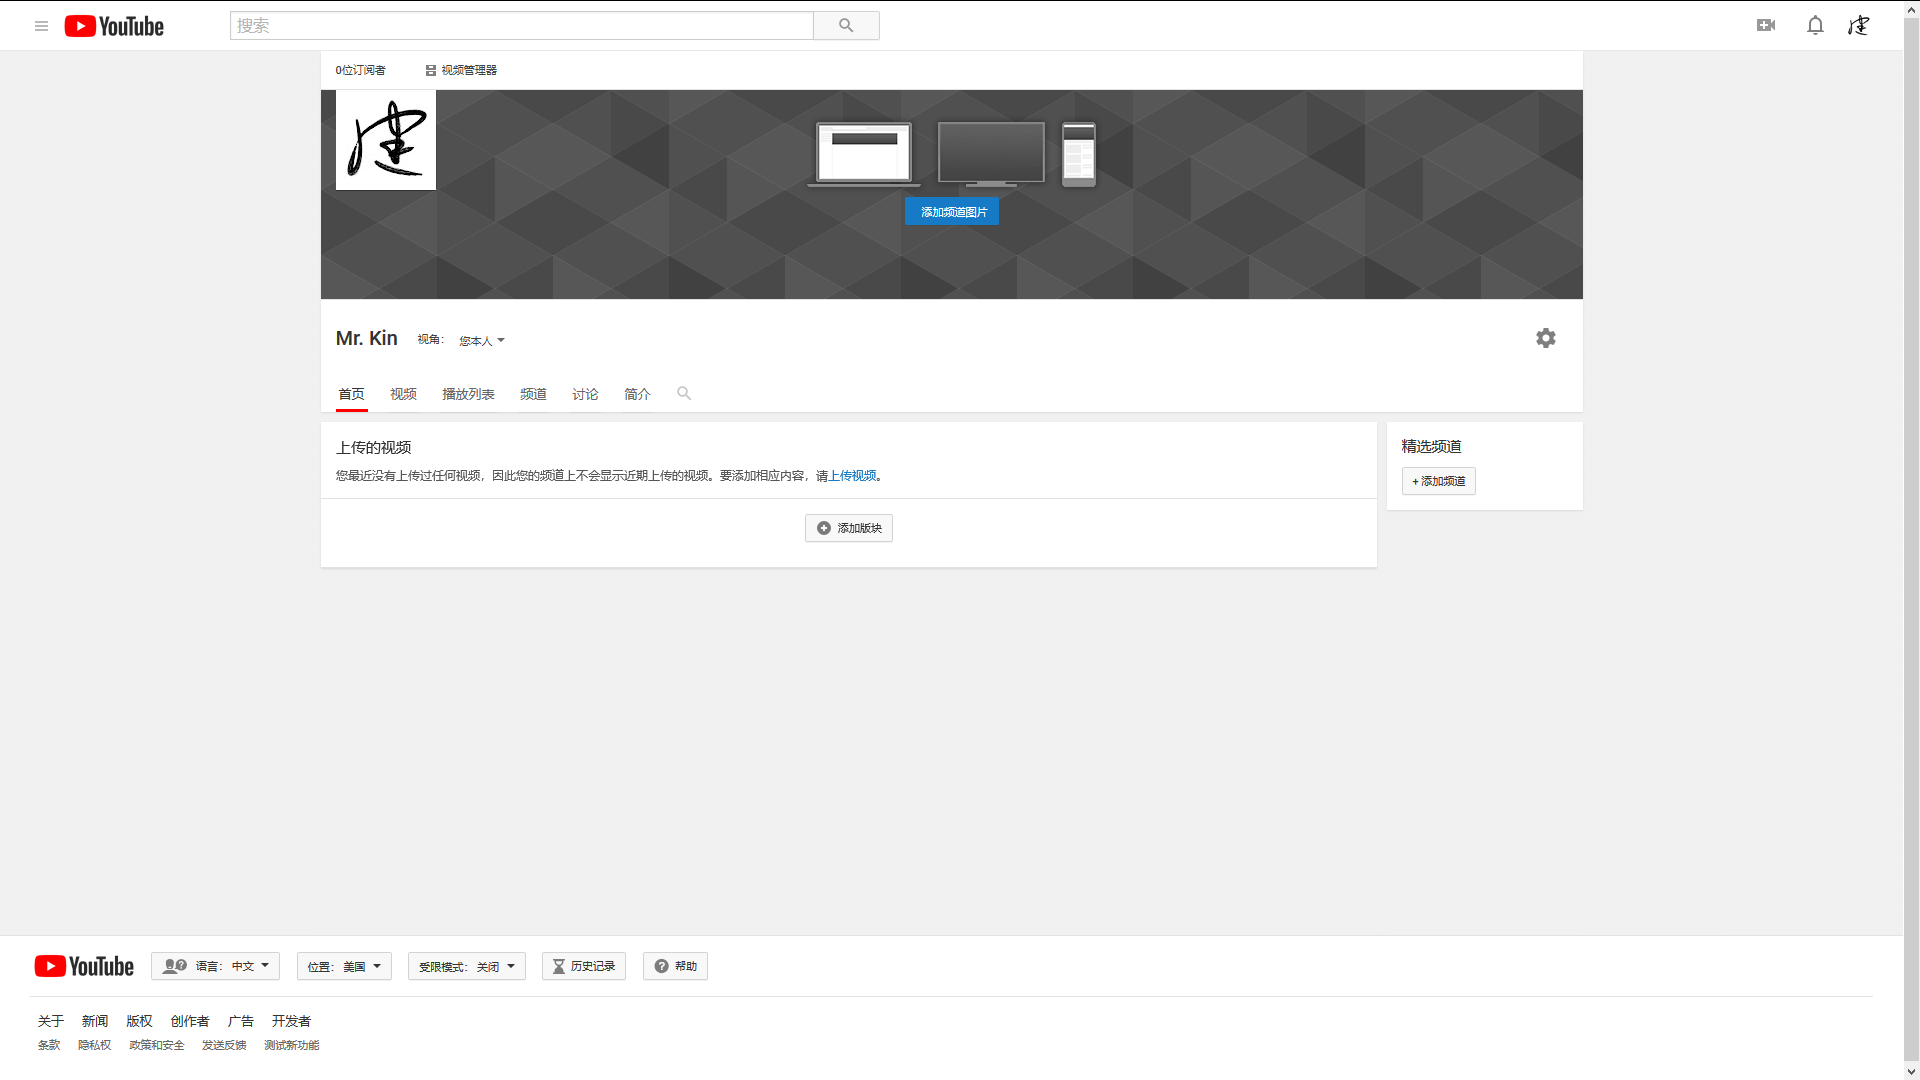
\includegraphics[scale=0.055]{Youtube}
    \end{minipage}
\end{figure}
 % 出于特殊的安全设置,\include 命令无法使用相对路径,因为需要读写权限以给 included file 写 aux 文件,而 \input 命令只需要读权限。
    \clearpage
    \phantomsection
\begin{center}
    {\bfseries\sffamily\Large 版权声明}
\end{center}
\addcontentsline{toc}{chapter}{版权声明}

\noindent 作者:Mr. Kin \\
\DetectToksEmpty\LinkBlogPost
\ifToksEmpty
博文链接:链接暂空\\
\else
博文链接:\href{\the\LinkBlogPost}{跳转博文页}\\
\fi
\DetectToksEmpty\LinkPDFSource
\ifToksEmpty
PDF及LaTex源码链接:链接暂空\\
\else
PDF及LaTex源码链接:\href{\the\LinkPDFSource}{跳转PDF及LaTex源码页}\\
\fi
\DetectToksEmpty\LinkVideo
\ifToksEmpty
\else
相关视频创作链接:\href{\the\LinkVideo}{跳转视频页}\\
\fi
许可协议:本作品的所有内容,除个人设计创作的图像(如logo等)和相关的视频创作及其他特别声明外,均采用\href{https://creativecommons.org/licenses/by-nc-sa/4.0/deed.zh}{知识共享\ 署名-非商业性使用-相同方式共享 4.0 国际许可协议}进行发布。版权 © Mr. Kin,保留所有权利。
\includegraphics[scale=.4]{CC-BY-NC-SA}\\*[1.3ex]
\begin{tabular}{|*{3}{p{0.306\textwidth}|}}
    \hline
    \textsf{\bfseries 允许} & \textsf{\bfseries 限制} & \textsf{\bfseries 条件} \\
    \hline
    \vspace{-8pt}{\color{green}√} 修改 & \vspace{-8pt}{\color{red}×} 商标使用 & \vspace{-8pt}{\color{blue}$\odot$} 保留原署名 \\[-12pt]
    {\color{green}√} 分发 & {\color{red}×} 专利使用 & {\color{blue}$\odot$} 状态变更说明 \\[-12pt]
    {\color{green}√} 个人使用 & {\color{red}×} 商业使用 & {\color{blue}$\odot$} 相同的许可和版权声明 \\
    \hline
\end{tabular}
\\*[1.3ex]
\emph{注:若想对本作品进行转载、引用亦或是进行二次创作时,请详细阅读上述相关协议内容(若不理解,请点击链接跳转阅读)。为保障本人权利,对于违反者,本人将依法予以处理!望周知!——Mr. Kin}

\begin{center}
    {\bfseries\sffamily\Large 勘误声明}
\end{center}

虽本人写作时已尽力保证其内容的正确性,但因个人知识面和经验的局限性以及计算机技术等相关技术日新月异,本作品内容或存在一些错误之处。还望诸君发现错误后能够\hyperlink{contact}{联系我}以更正错误,不胜感激!——Mr. Kin

\begin{center}
    {\bfseries\sffamily\Large 侵权声明}
\end{center}

若本作品采用的第三方内容侵犯了你的版权,请与我\hyperlink{contact}{联系}进行处理,谢谢!——Mr. Kin

\begin{center}
    {\bfseries\sffamily\Large 第三方开源许可声明}
\end{center}

\noindent 本作品使用的第三方开源产品有:
\begin{multicols}{2}
\begin{itemize}
    \item \href{https://github.com/adobe-fonts}{Adobe Fonts}: \href{https://github.com/adobe-fonts/source-serif-pro/blob/release/LICENSE.md}{OFL v1.1}
    \item \href{https://tug.org/texlive/}{Tex Live}: \href{https://tug.org/texlive/copying.html}{TeX Live Licensing}
    \item \href{https://code.visualstudio.com/}{Visual Studio Code}: \href{https://github.com/Microsoft/vscode/blob/master/LICENSE.txt}{MIT}
    \item \href{http://ffmpeg.org/}{FFmpeg}: \href{http://ffmpeg.org/legal.html}{LGPL v2.1 / GPL v2}
    \item \href{https://krita.org/en/}{Krita}: \href{https://docs.krita.org/en/KritaFAQ.html?highlight=license#license-rights-and-the-krita-foundation}{Krita's GPL license}
    \item \href{https://inkscape.org/}{Inkscape}: \href{https://inkscape.org/about/license/}{GPL}
    \item \href{https://www.gimp.org}{GIMP}: \href{https://www.gimp.org/about/COPYING}{GPL}
    \item \href{https://www.blender.org}{Blender}: \href{https://www.blender.org/about/license/}{GPL}
    \item \href{https://www.audacityteam.org/}{Audacity}: \href{https://www.audacityteam.org/about/license/}{GPL v2}
    \item \href{https://handbrake.fr}{Handbrake}: \href{https://github.com/HandBrake/HandBrake/blob/master/LICENSE}{GPL v2}
\end{itemize}
\end{multicols}

\noindent 更多请点击查看\href{https://mister-kin.github.io/about/third-party-declaration/}{第三方声明页}!

    \clearpage
    {\centering \tableofcontents} % 生成目录页。
    \mainmatter

    % 正文
    \chapter{考试大纲}

\begin{intro}
    政治、英语、数学这三个公共课是全国统考,专业课只有法硕、农学、教育学、心理学、历史学、西医综合、计算机是全国统考,其他的都是学校自主出题。
\end{intro}

\noindent {\bfseries \sffamily 成绩线}
待查询。

\section{考试及试题信息}
\subsection{数学一}
\paragraph{试卷情况} 分值150,考试时长180min。
\paragraph{内容占比} 56\%高等数学(微积分),22\%线性代数,22\%概率论与数理统计。
\paragraph{题型结构:}
\begin{enumerate}
    \item 单项选择8道,共32分
    \item 填空题6道,共24分
    \item 解答题(含证明题)9道,共94分
\end{enumerate}

\subsection{英语一}
\paragraph{试卷情况} 分值100,考试时长180min。
\paragraph{内容}词汇(5500+附表词汇);语法(基本熟练地运用基本的语法知识)。
\paragraph{题型结构:}
\begin{enumerate}
    \item 英语知识运用(10分)
    \begin{enumerate}
        \item 20道完形填空(四选一):1篇文章(240~280词),词汇、语法和结构。
    \end{enumerate}
    \item 阅读理解(40+10+10分)
    \begin{enumerate}
        \item 20道多项选择(四选一):4篇文章(共约1600词),理解主旨要义、具体信息、概念性含义、进行判断、推理和引申,根据上下文推测生词词义。
        \item 5道选择搭配:1篇文章(500~600词),理解连贯性、一致性等语段特征和文章结构。
        \item 5道英译汉:1篇文章(400词,5个划线部分约150词),理解复杂概念、结构。
    \end{enumerate}
    \item 写作(10+20分)
    \begin{enumerate}
        \item 一个应用文写作(规定情景:信函、备忘录、报告等):100词。
        \item 一个短文写作(描述性、叙述性、说明性、议论性文章):160~200词。
    \end{enumerate}
\end{enumerate}

\subsection{政治}
\paragraph{试卷情况} 分值100,考试时长180min。
\paragraph{内容占比} 24\%马原,30\%毛中特,14\%史纲,16\%思修,16\%时政和当代。
\paragraph{题型结构:}
\begin{enumerate}
    \item 单项选择16道:16分
    \item 多项选择17道:34分
    \item 材料分析题:50分
\end{enumerate}

\subsection{408}
\paragraph{试卷情况} 分值150,考试时长180min。
\paragraph{内容占比} 数据结构(45分),计算机组成原理(45分),操作系统(35分),计算机网络(25分)。
\paragraph{题型结构:}
\begin{enumerate}
    \item 单项选择40道:80分
    \item 综合应用题:70分
\end{enumerate}

\section{复习规划}
学习纲要:学习完一节知识后进行复盘记录。

\subsection{数学}
\paragraph{复习资料} 线代李永乐、高数汤家凤/武忠祥,概率王式安。

\begin{enumerate}
    \item
\end{enumerate}

\subsection{政治}
\paragraph{复习资料} 《精讲精练》《1000题》《八套卷》《四套卷》《风中劲草》《模拟卷》

\subsection{408}

    \chapter{数学一}

\section{线性代数}
\begin{intro}
    六大块:行列式、矩阵、向量、方程组、特征值、二次型。其中\textbf{方程组}和\textbf{特征值}为重点。
\end{intro}

\subsection{行列式(Determinant)}
\subsubsection{考纲}
考纲内容:行列式的概念和基本性质;行列式按行(列)展开定理

考纲要求:了解行列式概念,掌握行列式性质;能运用行列式性质和定理计算

$
\begin{vmatrix}
    a_{11} & a_{12} \\
    a_{21} & a_{22} \\
\end{vmatrix}
$test


    \chapter{408专业课}

\section{计算机组成原理}
\begin{intro}
    计算机的信息由二进制表示,传递由电路实现,其中低/高电平表示二进制中的0/1。
\end{intro}

\subsection{计算机系统概述}



    \nocite{*} % 不使用 cite 也能生成参考文献。
    \printbibliography % 生成参考文献排版。
    \addcontentsline{toc}{chapter}{参考文献} % 添加参考文献进目录。

    \appendix
    % 附录

\end{document}
